\documentclass[aspectratio=169,10pt]{beamer}\usetheme{default}\usecolortheme{seahorse}\setbeamertemplate{navigation symbols}{}\setbeamertemplate{footline}[frame number]
\usepackage[T1]{fontenc}\usepackage[utf8]{inputenc}\usepackage{helvet}\usepackage{booktabs,amsmath}
\title{How many people cycle rue de Terrebonne in winter, and how often?}\subtitle{Bicycle counts on four sensors, a frequency distribution, and the APC-NDG survey in context}\author{Terrebonne-open-sources (a resident of Côte-des-Neiges--Notre-Dame-de-Grâce)}\date{2026-11-07}
\begin{document}
\begin{frame}\titlepage\end{frame}
\begin{frame}{Two units}\begin{itemize}
\item Counters count \textbf{passages}: one bicycle, one point, one direction. The survey counts \textbf{people}.
\item Exposure and use accrue per passage; representation is counted in persons. Neither converts into the other without an assumption on how often each person rides and whether a trip crosses the point twice.
\item Questions: what does the structure of the counts say about frequent and occasional riders? What bounds on individuals follow? How do the survey\textquoteright{}s 87 winter cyclists (36 at least weekly) sit against the counts?
\end{itemize}\end{frame}
\begin{frame}{Four sensors, two winters}\centering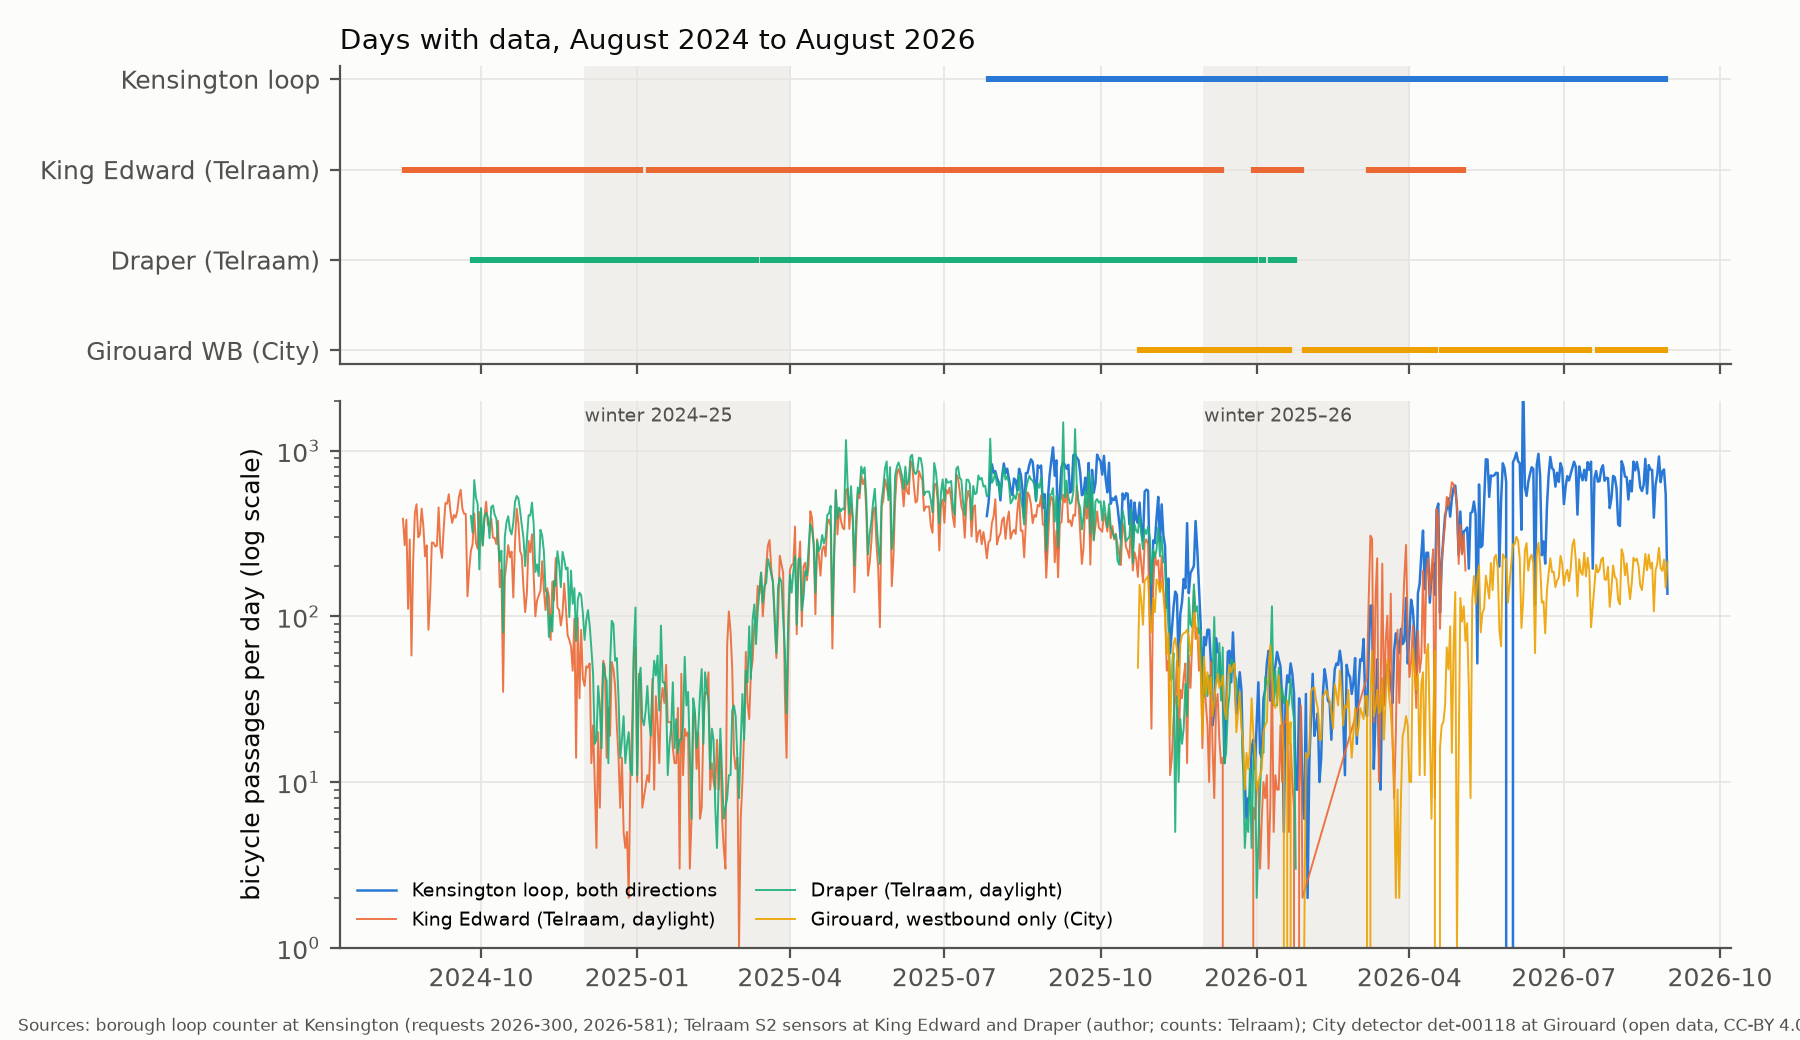
\includegraphics[width=0.9\textwidth]{figures/coverage_and_series_en.png}\end{frame}
\begin{frame}{Data and caveats}\begin{itemize}
\item \textbf{Kensington loop} (borough): hourly by direction, Jul 2025--May 2026; westbound channel degraded from March 2026 $\Rightarrow$ core period Dec 1, 2025 -- Feb 28, 2026.
\item \textbf{King Edward} and \textbf{Draper} (Telraam S2, the author\textquoteright{}s): hourly, daylight only, uptime per hour; Draper stopped Jan 24, 2026; counts belong to Telraam, aggregates only.
\item \textbf{Girouard} (City det-00118): westbound only, from Oct 23, 2025 (open data).
\item \textbf{Miovision} one-day counts: Sept 19, 2024 and Jan 29, 2025 (requests 2026-581, 2026-634).
\item ECCC daily weather; computed sunrise and sunset.
\end{itemize}\end{frame}
\begin{frame}{The winter at Kensington, Dec 1 -- Feb 28}\begin{columns}\column{0.55\textwidth}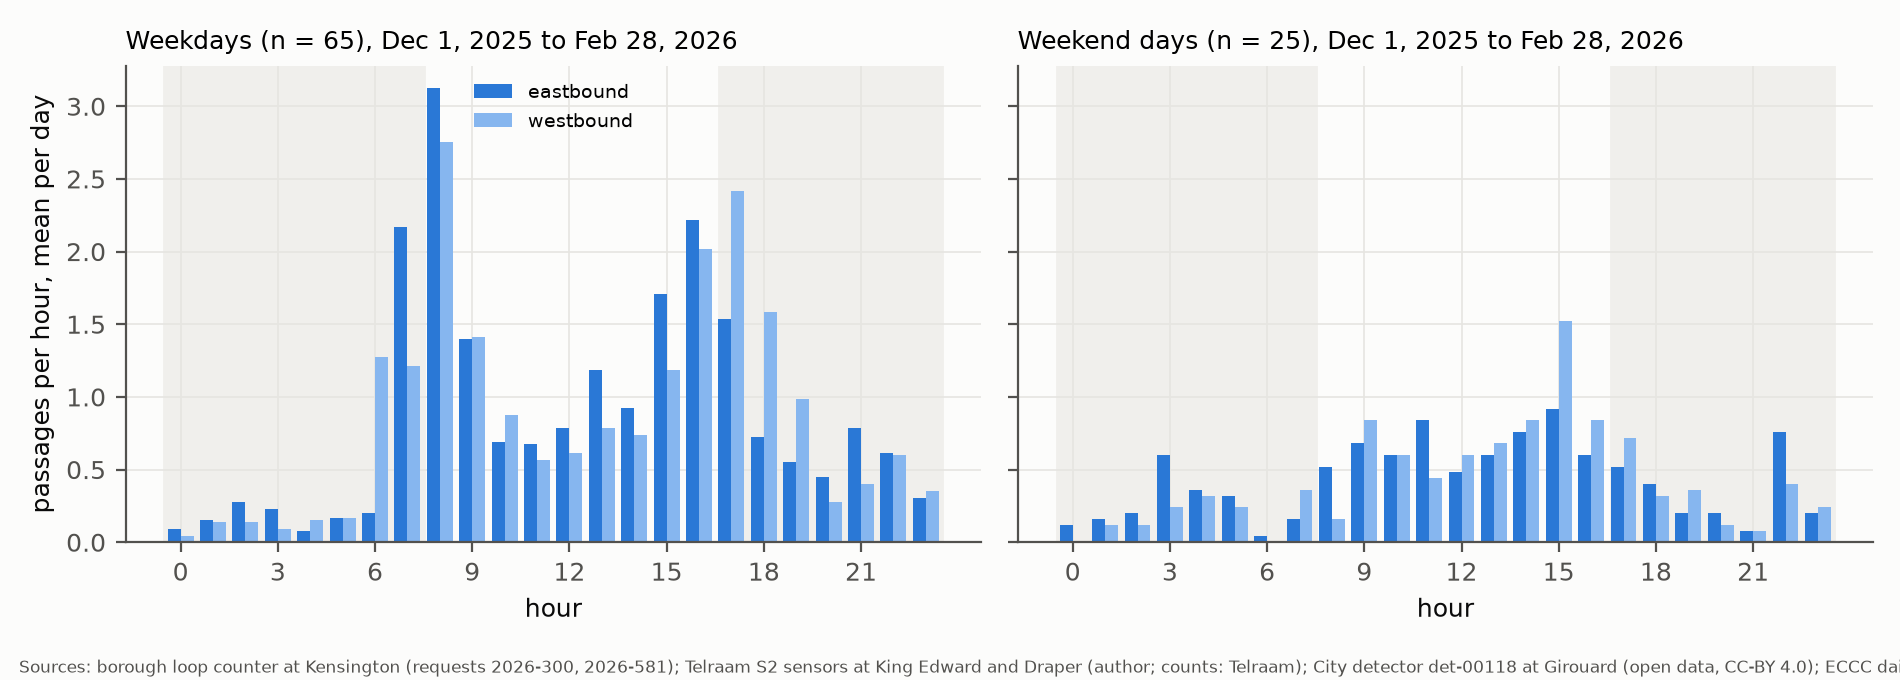
\includegraphics[width=\textwidth]{figures/kensington_hourly_profile_en.png}\column{0.45\textwidth}\small\begin{itemize}
\item 3,232 passages in 90 days; weekdays 41.8 (p10--p90 17--62), weekend 20.5.
\item Mild weekdays 50.6, harsh 40.1, holiday 22.0.
\item Matched AM/PM round trips: 11.0 per weekday, 53\,\% of weekday passages.
\item 41\,\% of passages in darkness.
\item Dec 1 -- Mar 31: 4,891 passages, no day below 2, 60 days $\geq 40$ (lower bound).
\end{itemize}\end{columns}\end{frame}
\begin{frame}{Weather and round trips}\centering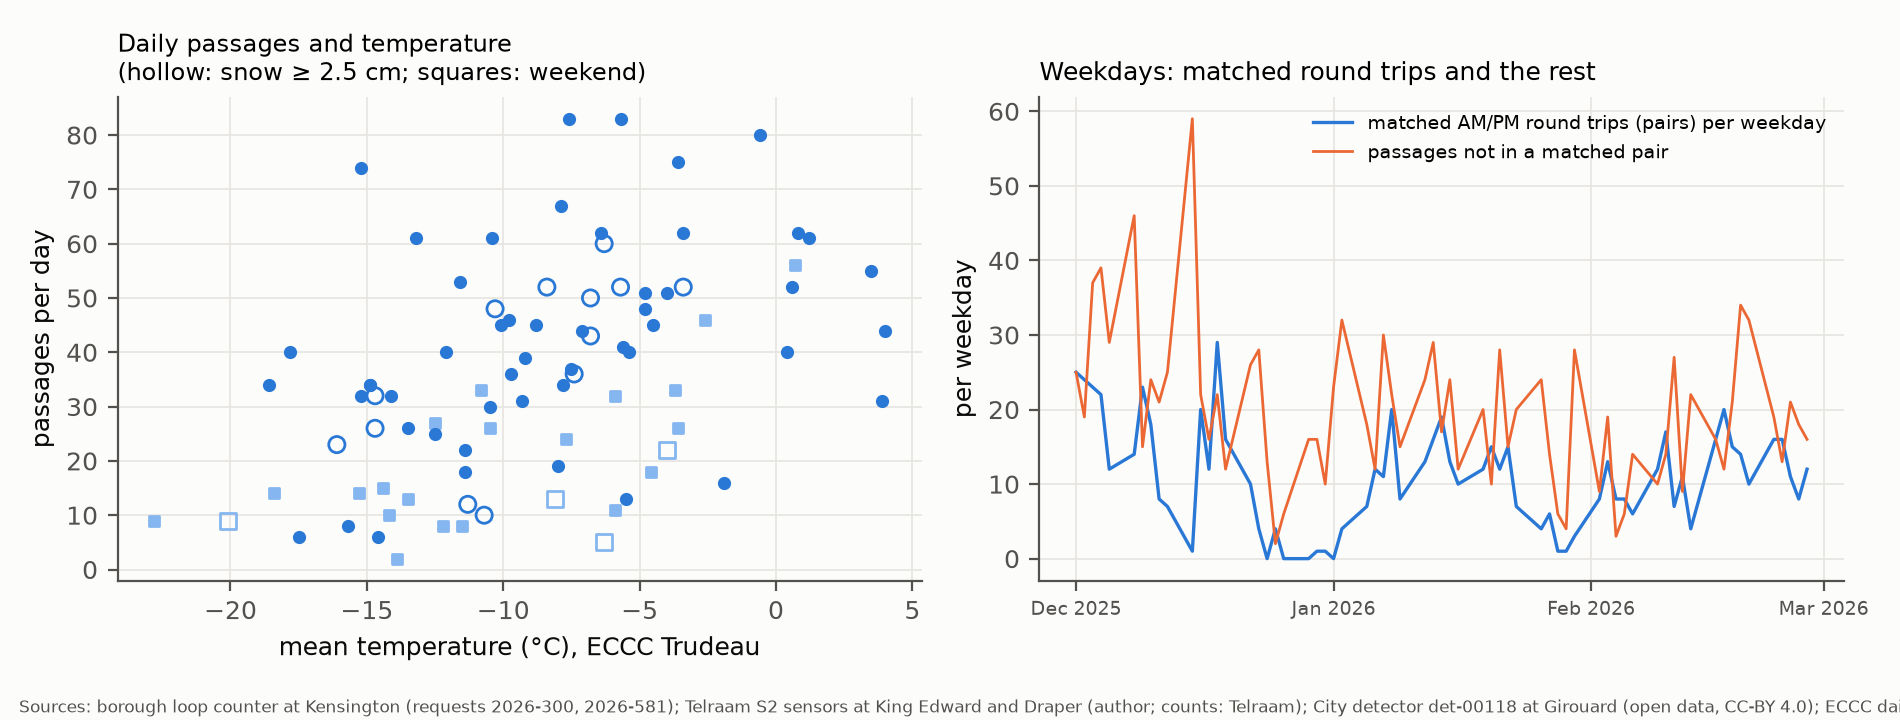
\includegraphics[width=0.95\textwidth]{figures/kensington_weather_pairs_en.png}\\{\scriptsize NB regression: weekend -49 \%, holiday period -41 \%, +3 \% per unit of mean temperature, -2 \% per unit of snow on the ground; residual lag-1 autocorrelation 0.182.}\end{frame}
\begin{frame}{The other points: the east end holds up in winter}\centering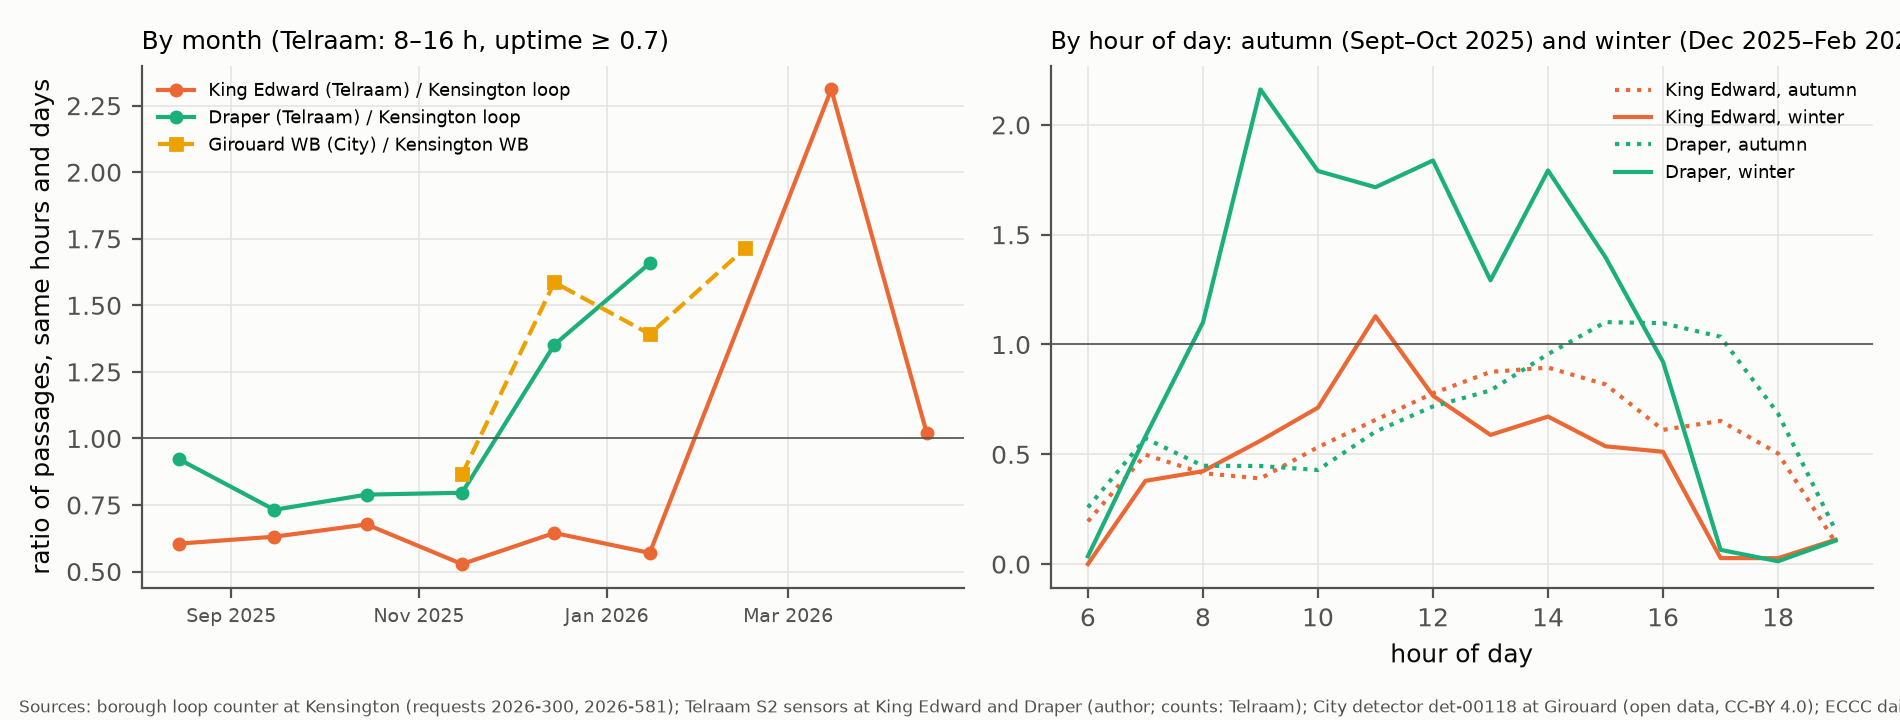
\includegraphics[width=0.95\textwidth]{figures/cross_sensor_ratios_en.png}\\{\scriptsize Dry days, winter core: King Edward 0.57, Draper 1.33 of the loop; Girouard WB 1.58 of the loop\textquoteright{}s WB (0.86 in November).}\end{frame}
\begin{frame}{Snow days: the instruments diverge}\centering\small\begin{tabular}{@{}llrrrrr@{}}\toprule sensor & weather & days & matched h & Telraam & Kensington & ratio\\ \midrule
King Edward & no snow & 15 & 129 & 185 & 322 & 0.575 \\
King Edward & snow ge 2.5cm & 13 & 117 & 204 & 231 & 0.883 \\
King Edward & mild & 16 & 141 & 203 & 442 & 0.459 \\
King Edward & harsh & 27 & 229 & 351 & 480 & 0.731 \\
Draper & no snow & 23 & 187 & 611 & 459 & 1.331 \\
Draper & snow ge 2.5cm & 12 & 96 & 405 & 190 & 2.132 \\
Draper & mild & 24 & 188 & 747 & 582 & 1.284 \\
Draper & harsh & 28 & 222 & 789 & 467 & 1.69 \\
\bottomrule\end{tabular}\\[6pt]\footnotesize On days with $\geq 2.5$ cm of snow both Telraam sensors count 50--60\,\% more relative to the loop. Either the camera over-detects on snow days, or cyclists leave the snowed-in lane for the roadway where the loop cannot see them. The data do not settle it; dry-day ratios are used, and the loop\textquoteright{}s snow-day counts may be low.\end{frame}
\begin{frame}{Two snapshot days}\centering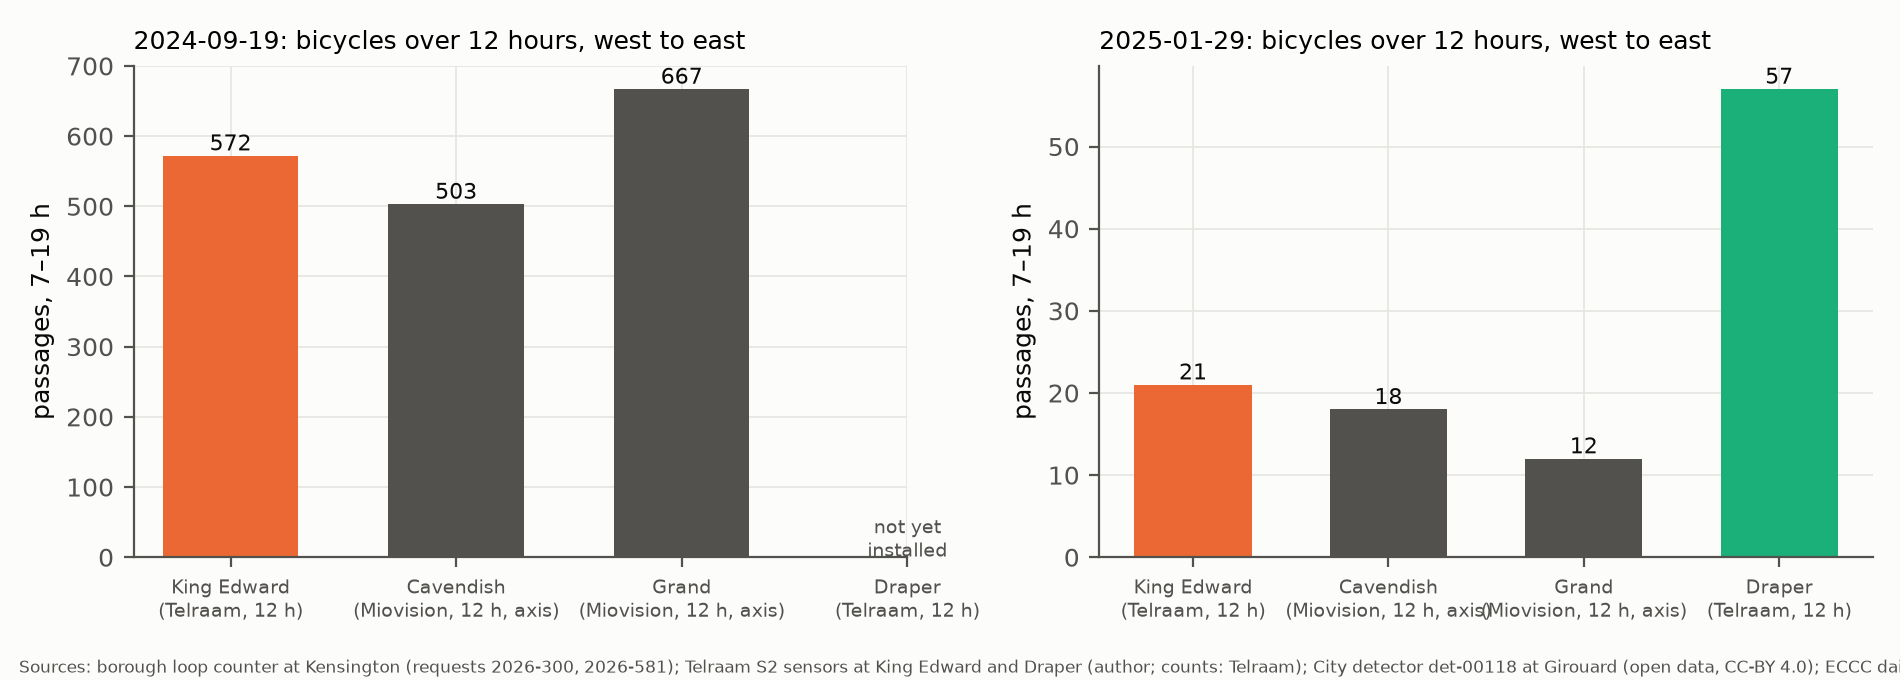
\includegraphics[width=0.95\textwidth]{figures/snapshot_days_en.png}\\{\scriptsize Jan 29, 2025: 7.4 cm of snow, mean -11.5 $^\circ$C. Grand: 8 eastbound, 0 westbound in six peak hours (the « 8 »): no return leg in the window. Draper is a snow-day Telraam count.}\end{frame}
\begin{frame}{Floors under the number of individuals (no model)}\centering\small\begin{tabular}{@{}llrrrl@{}}\toprule point & date & passages & people, $m=2$ & people, $m=4$ & note\\ \midrule
Kensington loop & 2026-03-30 & 129 & 65 & 33 & WB channel degraded\\
Kensington, core & 2025-12-03 & 83 & 42 & 21 & both channels sound\\
King Edward (Telraam) & 2026-03-09 & 307 & 154 & 77 & daylight, no snow\\
Girouard WB (City) & 2026-01-09 & 67 & 34 & 17 & one direction\\
\bottomrule\end{tabular}\\[6pt]\footnotesize If no one crosses a point more than $m$ times in a day, the largest day divided by $m$ is a floor under the distinct cyclists of the winter.\end{frame}
\begin{frame}{A frequency-band model}\small
\[ Y_d \sim \mathrm{NB}\Big(\sum_b N_b\, p_b(d)\, c_b\Big), \qquad P_d \sim \mathrm{NB}\Big(\sum_b N_b\, p_b(d)\, \pi_b\Big) \]
\begin{itemize}
\item Three bands (most weekdays / 1--3 days a week / a few times a month), each a template: probability of riding by day type and weather, passages per riding day, share of riding days giving a matched pair.
\item Fitted by maximum likelihood on the core period (daily totals and matched pairs); 95\,\% profile intervals; four template sets.
\item Purpose: to show which quantities one counter determines and which it does not.
\end{itemize}\end{frame}
\begin{frame}{What the counts pin down, and what they do not}\centering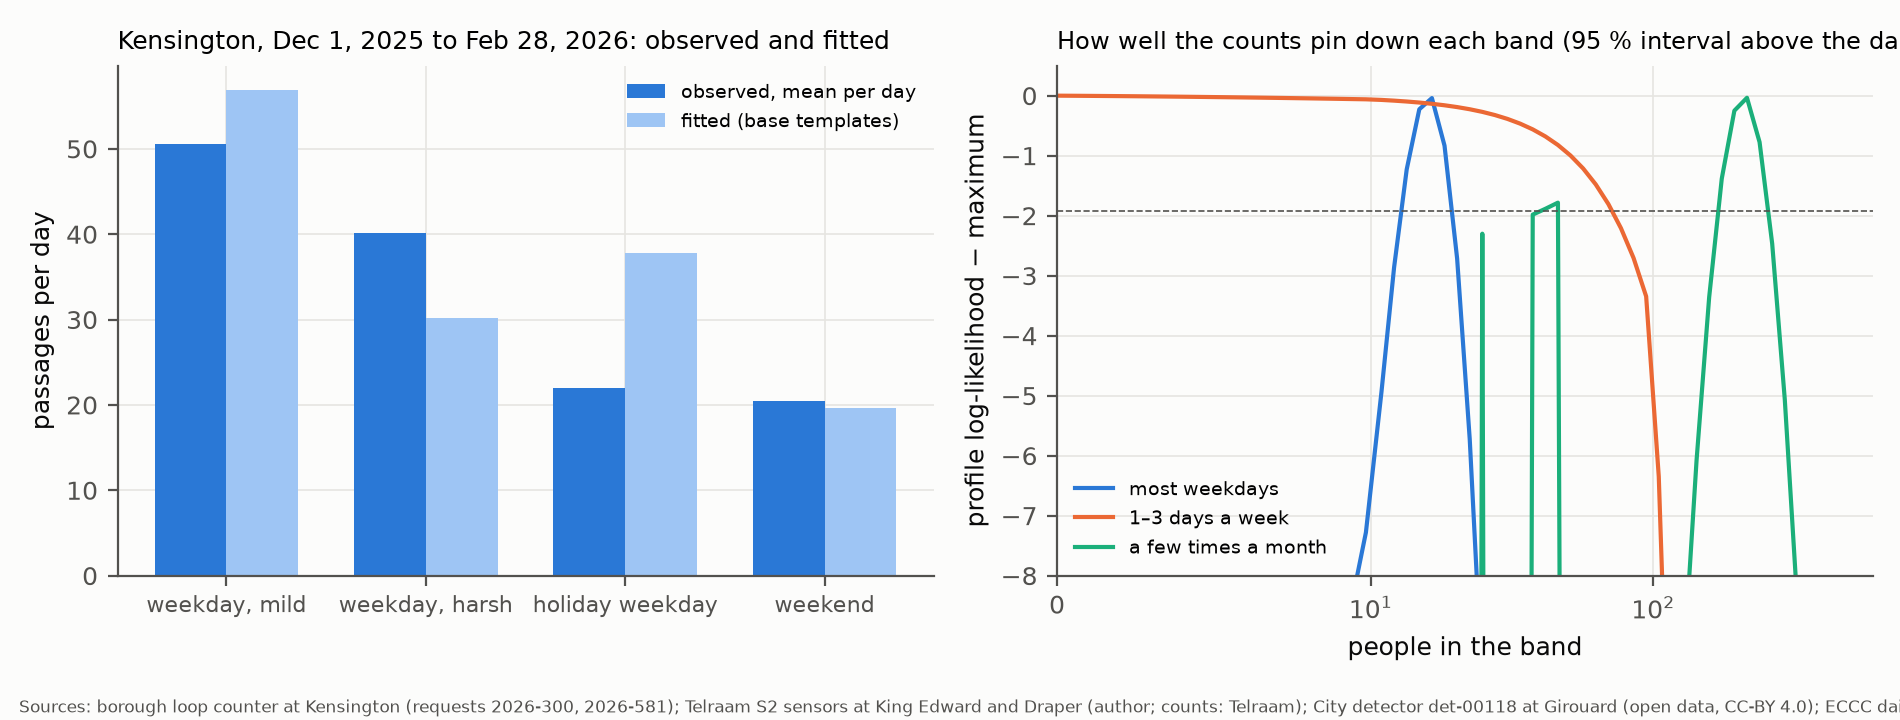
\includegraphics[width=0.95\textwidth]{figures/band_fit_en.png}\end{frame}
\begin{frame}{People per band, by template set (Kensington, core period)}\centering\scriptsize\resizebox{\textwidth}{!}{\begin{tabular}{@{}lllllrr@{}}\toprule templates & most weekdays & 1--3 days/week & frequent (both) & a few times a month & passages, frequent & fitted total\\ \midrule
base & 0 (0--10) & 61 (22--69) & \textbf{61} (32--70) & 66 (25--128) & 78\,\% & 3,151 \\
more one-way trips & 0 (0--12) & 73 (16--85) & \textbf{73} (29--85) & 88 (37--175) & 76\,\% & 3,118 \\
tail more weather-sensitive & 15 (10--16) & 0 (0--37) & \textbf{15} (12--48) & 253 (158--292) & 41\,\% & 3,380 \\
survey categories literal & 0 (0--11) & 41 (0--46) & \textbf{41} (11--48) & 173 (128--238) & 56\,\% & 3,225 \\
\bottomrule\end{tabular}}\\[6pt]\footnotesize Stable: the frequent core is small in number (11--85) and makes most of the passages. Not identified: the split daily / near-daily, and the size of the tail (25--292) without an assumption on how often an occasional rider rides.\end{frame}
\begin{frame}{From Kensington to the street}\begin{itemize}
\item Dry-day ratios to Kensington: King Edward 0.57, Draper 1.33, Girouard WB 1.58.
\item Trips crossing at least one point: between 1.58 (every trip crosses every point) and 4.48 (no trip crosses two) times the Kensington count.
\item Kensington is not the busiest point of the lane in winter; a count there is a lower bound on the street.
\item Year over year on common dates: King Edward 0.77, Draper 0.81 of the 2024--25 winter.
\end{itemize}\end{frame}
\begin{frame}{The survey in context}\begin{columns}\column{0.5\textwidth}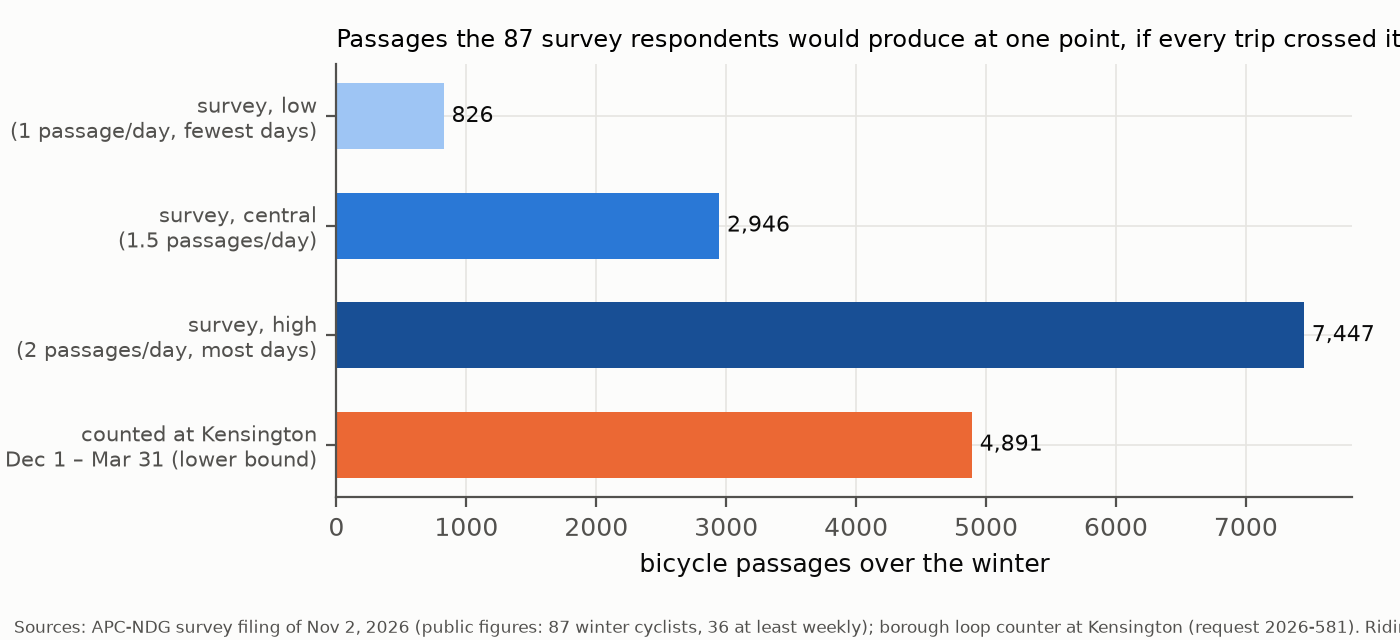
\includegraphics[width=\textwidth]{figures/survey_vs_count_en.png}\column{0.5\textwidth}\small\begin{itemize}
\item 87 respondents cycled on Terrebonne last winter, 36 at least weekly (public filing, Nov 2, 2026).
\item Their passages at one point, if every trip crossed it: 2,946 central (826--7,447) against 4,891 counted: 60\,\%.
\item 36 weekly riders against a frequent core of 11--85 at Kensington alone; 51 occasional against a tail of 25--292; both $\times$ the corridor factor for the street.
\item The survey reached a large share of frequent riders and a small share of the tail: the signature of a voluntary survey of users. The count does not contradict it; the 87 are a floor, not a measure.
\end{itemize}\end{columns}\end{frame}
\begin{frame}{What this settles and what it does not}\begin{itemize}
\item Trips at stake: 4,891 passages at one point over the proposed window, more over the street.
\item People: at least 154 at King Edward on one March day and 42 at Kensington on one December day, before any assumption; beyond that, the head count depends on the frequency assumed, and a division of passages by two is one such assumption.
\item About 11 round-trip commuters cross Kensington on an ordinary winter weekday; frequent riders make most passages; the tail is large in people and poorly measured.
\item Open: the snow-day divergence between the camera sensors and the loop; a passage-weighted frequency distribution (asking passing cyclists at the counting point) would turn passages into people without a model.
\item Code, data tables and every figure: \url{https://openmobilitydata.github.io/Terrebonne-open-sources/2026-winter-counts-user-frequency/}
\end{itemize}\end{frame}
\end{document}
